\section{Design and implementation details}

\subsection{Skiller multiplayer framework}
Due to the desire of developing a fully functional multiplayer game, the \emph{Skiller multiplayer framework} \cite{skiller} has been used. This is a third party COTS software, and its usage has sped up the development process. Registration was needed in order to gain access to the Skiller SDK. When the registration was done, a new game could be created, and an application ID, an application key, and an application secret was supplied. These are used in the code to identify the specific application. \\

This framework supplies a server solution for turn based games, and it has been implemented in the network class. When playing a network game, the GameController class tells the Game model to  network class sends event messages to the server, and the server delivers it to the opponent.

\subsection{Activities}
Figure \ref{fig:activities} shows an overview of the application's different activities, and how the user interactions can change them. The user can navigates back to the menuActivity by pressing the back button.\\

\begin{figure}[H]
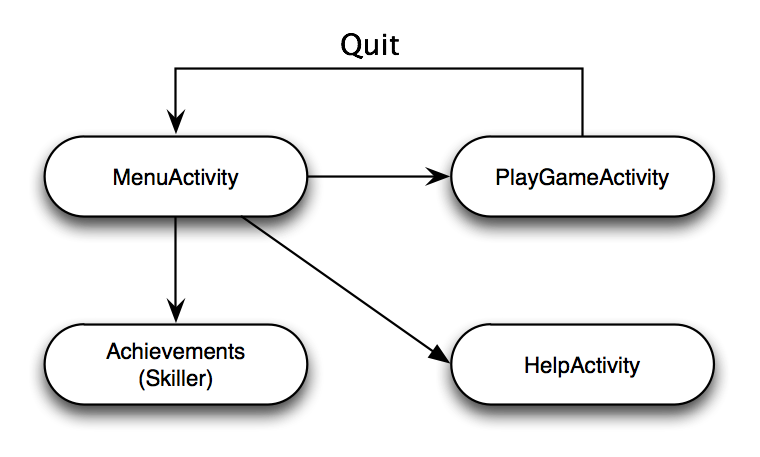
\includegraphics[width=1\textwidth]{Images/activities}
\caption{Application activities}
\label{fig:activities}
\end{figure}

The MenuActivity shows a menu consisting of five items, allowing the user to create or join a multiplayer game, start a local game, check achievements, or check the game rules. The PlayGameActivity is responsible for creating or joining multiplayer games, and starting local games. The HelpActivity is responsible for showing the game rules. The achievement screen is supplied by \emph{Skiller}.\\

Screencaps of the different activities, and the achievement screen, are shown in section \ref{section:playing}.

\subsection{MVC}

Our implementation of the MVC structure is based interface communication. In regular Java it is more common to create a MVC structure where the view has model and the controller contains view and model. Android has its own MVC structure where an activity represent controller and view, which makes it difficult to build on the MVC in a regular way. The most favorable way of createing MVC in android is to use interfaces to update the view when there are changes in the model. Figure~\ref{fig:mvc} shows an overview of the MVC structure, with BoardView (View), GameController (Controller) and Game (Model). When the user interact with the view the controller handles the user action and tells the model what to do. When the model is updated, the view receive a message via the interface, and updates the screen.

\begin{figure}[H]
\begin{center}
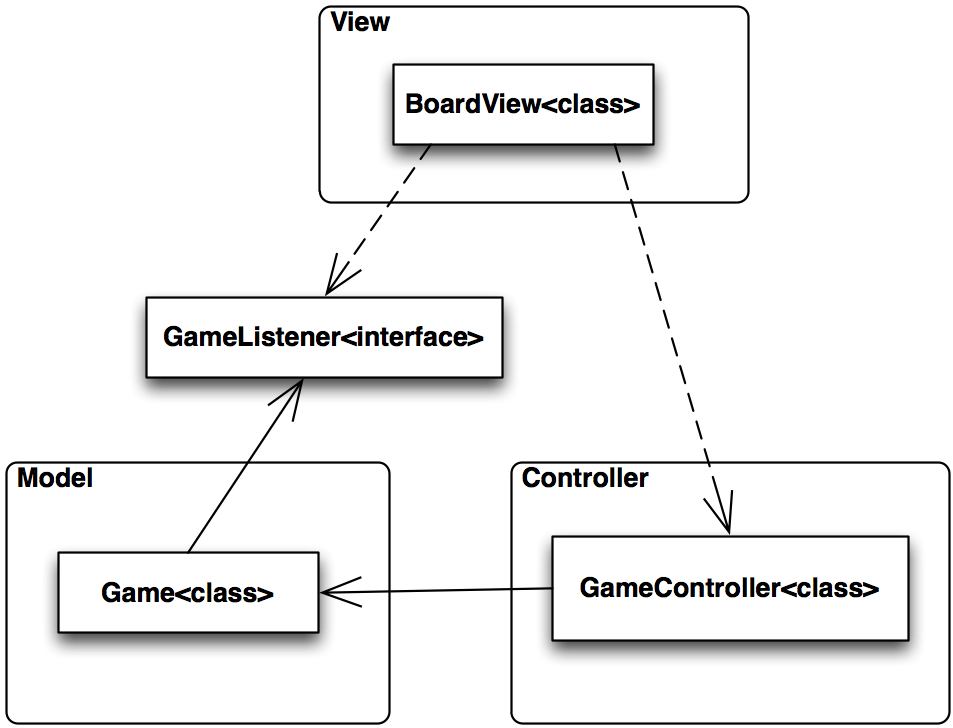
\includegraphics[width=0.7\textwidth]{Images/mvc}
\caption{MVC structure}
\label{fig:mvc}
\end{center}
\end{figure}

\subsection{States}

The Game class is implemented with associated states. The states change on runtime depending on player interaction. All states have their own way of controlling user possibilities, and telling the user what to do while playing. Figure \ref{fig:states} shows the relation between the Game class, the State interface, and the context classes implementing the State interface.

\begin{figure}[H]
\begin{center}
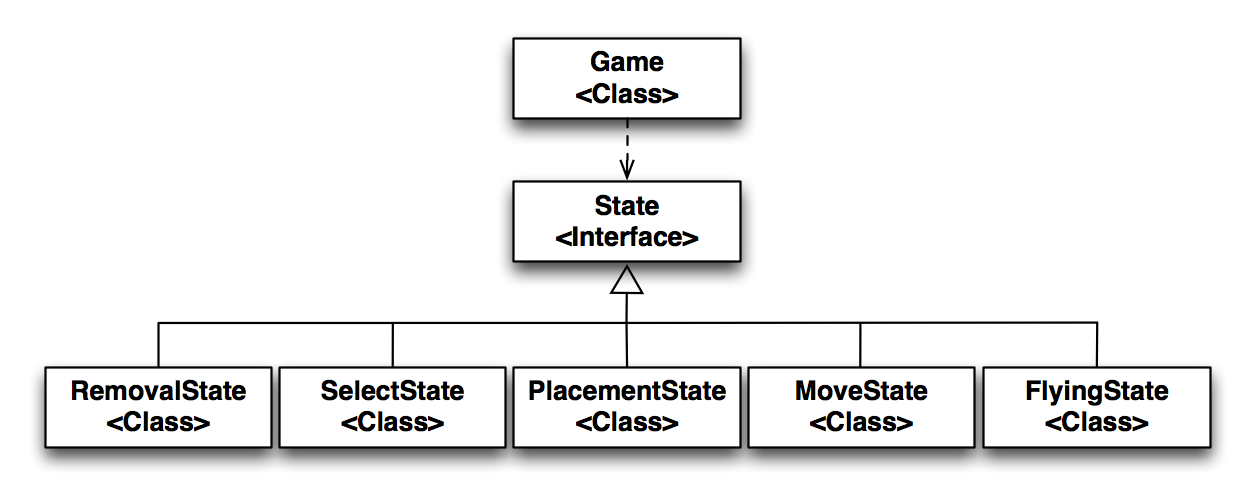
\includegraphics[width=\textwidth]{Images/states}
\caption{State structure}
\label{fig:states}
\end{center}
\end{figure}

